\uuid{nQHm}
\titre{Étude des extremums d'une fonction de deux variables}
\theme{}
\auteur{Grégoire MENET}
\datecreate{2025-04-16}
\organisation{AMSCC}

\contenu{
	
	\texte{
		On considère la fonction \( f \) définie par \( f(x,y)=x^2+y \) sur l'ensemble :
$$
		\mathcal{K}=\left\{\left.(x,y)\in\R^2\right|\ x^2+y^2\leq1\ \text{et}\ x+y\geq0\right\}.
$$

On définit également les ensembles : $$B_1=\left\{ (x,-x) \in \mathbb{R}^2 \,,\,\ x\in\left[-\frac{\sqrt{2}}{2};\frac{\sqrt{2}}{2}\right]\right\} \text{ et } B_2=\left\{(\cos\theta,\sin\theta)\in \mathbb{R}^2 \,,\, \theta\in\left[-\frac{\pi}{4};\frac{3\pi}{4}\right]\right\}.$$
	}
	
	\begin{enumerate}
		\item \question{Représenter graphiquement  \(\mathcal{K}\). Le domaine \(\mathcal{K}\) est-il ouvert ? Est-il fermé ?}
		\indication{Tracer le disque unité défini par \(x^2+y^2\leq 1\) et la demi-plan défini par \(x+y\geq0\), puis représenter l'intersection de ces deux ensembles. Analyser les conditions sur le cercle (bord du disque) et la droite \(x+y=0\) pour déterminer la nature topologique de \(\mathcal{K}\).}
		\reponse{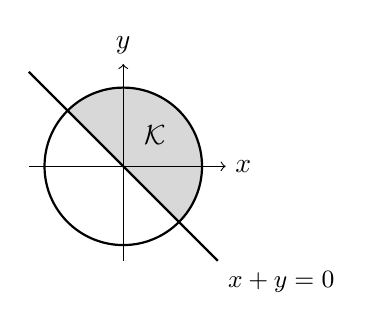
\begin{tikzpicture}[scale=1]
				% Disque unité
				\fill[white] (0,0) circle(1);
				
				% Demi-plan x + y >= 0
				\begin{scope}
					\clip (0,0) circle(1);
					\fill[gray!50, opacity=0.6] (-1.2,1.2) -- (1.2,-1.2) -- (1.2,1.2) -- cycle;
				\end{scope}
				
				% Cercle frontière
				\draw[thick] (0,0) circle(1);
				
				% Droite x + y = 0
				\draw[black, thick, ] (-1.2,1.2) -- (1.2,-1.2) node[below right] {\small $x + y = 0$};
				
				% Axes
				\draw[->] (-1.2,0) -- (1.3,0) node[right] {$x$};
				\draw[->] (0,-1.2) -- (0,1.3) node[above] {$y$};
				
				% Label du domaine
				\node at (0.4,0.4) { $\mathcal{K}$};
			\end{tikzpicture}
			Le domaine $\mathcal{K}$ est le disque unité tronqué par la droite $x + y = 0$. Il contient tout son bord, il est fermé et n'est pas ouvert. }
		\item \question{Justifier que $B_1$ et $B_2$ sont des sous-ensembles de $\mathcal{K}$ et les représenter sur le graphique. }
		\indication{Montrer que \(B_2\) est une portion du cercle unité correspondant aux angles \(\theta\in\left[-\frac{\pi}{4},\frac{3\pi}{4}\right]\) et préciser comment cette portion s'intersecte avec la condition \(x+y\geq0\).}
		\reponse{ $B_1$ est la partie du bord de $\mathcal{K}$ en forme d'arc de cercle ; $B_2$ est la partie droite. Les extrémités coïncident bien, ce sont les points de coordonnées respectives $\left(-\frac{\sqrt{2}}{2},\frac{\sqrt{2}}{2}\right)$ et $\left(\frac{\sqrt{2}}{2}, -\frac{\sqrt{2}}{2}\right)$. }
		\item \question{Justifier que la fonction \(f\) admet un maximum et un minimum global sur \(\mathcal{K}\).}
		\indication{Montrer que \(\mathcal{K}\) est un ensemble compact (fermé et borné) et appliquer le théorème des extrema sur les compacts pour conclure à l'existence d'un maximum et d'un minimum global de \(f\).}
		\reponse{On a que $\mathcal{K}$ est fermé borné et $f$ est continue (car polynomiale) sur ce domaine donc d'après le théorème des valeurs extrêmes, $f$ admet un maximum et un minimumm atteint sur $\mathcal{K}$. }
		
		\item \question{La fonction \(f\) admet-elle des points critiques ?}
		\indication{Rechercher, dans le domaine intérieur de \(\mathcal{K}\), les points où \(\nabla f=(0,0)\) et examiner l'existence de points critiques sur le bord si nécessaire.}
		\reponse{On calcule les dérivées partielles :
			\[
			\frac{\partial f}{\partial x}(x,y) = 2x,\quad \frac{\partial f}{\partial y}(x,y) = 1.
			\]
			Pour qu'un point soit critique, il faut que le gradient soit nul. Or ici :
			\[
			\frac{\partial f}{\partial y}(x,y) = 1 \neq 0,
			\]
			donc \( f \) n'a \textbf{aucun point critique à l'intérieur} de \( D_f \).}

		\item \question{Exprimer \(f(x,y)\) lorsque \((x,y) \in B_1\) en fonction d'une seule variable \(x\).}
			\indication{En substituant \(y=-x\) dans \(f\), on obtient \(f(x,-x)=x^2-x\). Préciser que \(B_1\) correspond à la droite d'équation \(y=-x\) limitée par l'intersection avec \(\mathcal{K}\).}
			\reponse{Si \( y = -x \), alors :
				\[
				f(x, -x) = x^2 - x.
				\]}
			
			\item \question{Dresser le tableau de variation de la fonction \(g: x\mapsto f(x,-x)\) sur \(\left[-\frac{\sqrt{2}}{2};\frac{\sqrt{2}}{2}\right]\).}
			\indication{Étudier la fonction \(g(x)=x^2-x\) sur l'intervalle donné en calculant sa dérivée, en déterminant les extrema locaux, et en présentant les variations sous forme de tableau.}
			\reponse{ On dérive $g(x)=f(x,-x)$.
				\[
				g'(x) = 2x - 1 \Rightarrow h'(x) = 0 \Leftrightarrow x = \frac{1}{2}.
				\]
				%Sur \( \left[-\frac{\sqrt{2}}{2}, \frac{\sqrt{2}}{2}\right] \approx [-0.707, 0.707] \), \( x = \frac{1}{2} \) appartient à l’intervalle.
				On a $\frac{1}{2} <\frac{\sqrt{2}}{2}$, on a donc le tableau suivant.
				\medskip
				
				\textbf{Tableau de variation :}
				
				\begin{center}
					\begin{tabular}{c|ccc}
						\( x \) & \( -\frac{\sqrt{2}}{2} \) & \( \frac{1}{2} \) & \( \frac{\sqrt{2}}{2} \) \\
						\hline
						\( g'(x) \) & $-$ & 0 & $+$ \\
						\( g(x) \) & $\searrow$ & $h(\frac{1}{2})$ & $\nearrow$ \\
					\end{tabular}
				\end{center}
				
				\textbf{Valeurs :}
				\[
				h\left(-\frac{\sqrt{2}}{2}\right) = \left(-\frac{\sqrt{2}}{2}\right)^2 - \left(\frac{\sqrt{2}}{2}\right) = \frac{1}{2} -\frac{\sqrt{2}}{2},
				\]
				\[
				h\left(\frac{\sqrt{2}}{2}\right) = \left(\frac{\sqrt{2}}{2}\right)^2 + \left(\frac{\sqrt{2}}{2}\right) = \frac{1}{2} +\frac{\sqrt{2}}{2},
				\]
				\[
				h\left(\frac{1}{2}\right) = \left(\frac{1}{2}\right)^2 - \frac{1}{2} = -\frac{1}{4}.
				\]}
			
			\item \question{On pose \(h(\theta)=f(\cos\theta,\sin\theta)\) pour tout $\theta\in\left[-\frac{\pi}{4};\frac{3\pi}{4}\right]$. Montrer que \(h'\) s'annule en \(\frac{\pi}{2}\) et en \(\frac{\pi}{6}\).}
			\indication{Calculer la dérivée de \(h(\theta)\) par rapport à \(\theta\) et résoudre l'équation \(h'(\theta)=0\) pour identifier les valeurs \(\theta=\frac{\pi}{2}\) et \(\theta=\frac{\pi}{6}\).}
			\reponse{On dérive :
				\[
				h'(\theta) = -2\cos\theta \sin\theta + \cos\theta = \cos\theta (1 - 2\sin\theta).
				\]
				Donc \( h'(\theta) = 0 \) ssi \( \cos\theta = 0 \) ou \( \sin\theta = \frac{1}{2} \).\\
				Sur $\left[-\frac{\pi}{4};\frac{3\pi}{4}\right]$ cela donne :
				\[
				\theta = \frac{\pi}{2}\ \ \text{ou}\ \ \theta = \frac{\pi}{6}.
				\]}
			
			\item \question{Dresser le tableau de variation de \(h\).}
			\indication{Étudier les variations de \(h(\theta)\) sur l'intervalle \(\left[-\frac{\pi}{4},\frac{3\pi}{4}\right]\) en utilisant les points critiques trouvés ainsi que les valeurs aux bornes.}
			\reponse{\begin{center}
					\begin{tabular}{c|ccccccc}
						\( \theta \) & \(-\frac{\pi}{4}  \) & &\( \frac{\pi}{6} \) & &\( \frac{\pi}{2} \) & &\(\frac{\pi}{4}  \)\\
						\hline
						\( \cos\theta \) & & $+$  &  &$+$ & 0 & $-$ &\\
						\hline
						\( 1 - 2\sin\theta \) & & $+$  & 0 &$-$ &  & $-$ &\\
						\hline
						\( h'(\theta) \) & & $+$  & 0 &$-$ &0  & $+$ &\\
						\hline
						\( h(\theta) \)  & & $\nearrow$ &  &$\searrow$ & &$\nearrow$ &\\
					\end{tabular}
				\end{center}
				%On étudie les signes de \( g'(\theta) = \cos\theta (1 - 2\sin\theta) \) sur \( \left[ -\frac{\pi}{4}, \frac{3\pi}{4} \right] \), avec annulations en \( \frac{\pi}{6} \) et \( \frac{\pi}{2} \).\\
				% On peut utiliser une analyse graphique ou numérique pour déterminer les variations (ou faire un tableau de signe de \( g' \)).\\
				
				On calcule les valeurs de \( g \) :
				\[
				g\left(\frac{\pi}{2}\right) = \cos^2\left(\frac{\pi}{2}\right) + \sin\left(\frac{\pi}{2}\right) = 0 + 1 = 1,
				\]
				\[
				g\left(\frac{\pi}{6}\right) = \cos^2\left(\frac{\pi}{6}\right) + \sin\left(\frac{\pi}{6}\right) = \left(\frac{\sqrt{3}}{2}\right)^2 + \frac{1}{2} = \frac{3}{4} + \frac{1}{2} = \frac{5}{4},
				\]
				\[
				g\left(-\frac{\pi}{4}\right) = \cos^2\left(-\frac{\pi}{4}\right) + \sin\left(-\frac{\pi}{4}\right) =\frac{1}{2}-\frac{\sqrt{2}}{2},
				\]
				\[
				g\left(\frac{\pi}{4}\right) = \cos^2\left(\frac{\pi}{4}\right) + \sin\left(\frac{\pi}{4}\right) =\frac{1}{2}+\frac{\sqrt{2}}{2}.
				\]		
			}
		
		\item \question{En utilisant les questions précédentes, déterminer le maximum et le minimum global de \(f\) sur \(\mathcal{K}\). En quels points ces extremums sont-ils atteints ?}
		\indication{Comparer les valeurs de \(f\) obtenues dans le domaine intérieur et sur le bord de \(\mathcal{K}\), en s'appuyant sur les études réalisées précédemment, pour identifier les points où \(f\) atteint son maximum et son minimum global.}
		\reponse{On ordonne les différentes valeurs trouvées. Notons que $\frac{1}{2}<\frac{\sqrt{2}}{2}<\frac{3}{4}$ (ce voit en prenant le carré par exemple). On a donc :
			$$-\frac{1}{4}<\frac{1}{2}-\frac{\sqrt{2}}{2}<1<\frac{1}{2}+\frac{\sqrt{2}}{2}<\frac{5}{4}.$$
			%C'est à dire :
			%$$f(\frac{1}{2},-\frac{1}{2})<\frac{1}{2}-\frac{\sqrt{2}}{2}<1<\frac{1}{2}+\frac{\sqrt{2}}{2}<\frac{5}{4}.$$
			Le minimum de $f$ est donc $-\frac{1}{4}$ et le maximum est $\frac{5}{4}$. Le minimum est atteint en $(\frac{1}{2},-\frac{1}{2})$ et le maximum est atteint en $\left(\cos\left(\frac{\pi}{6}\right),\sin\left(\frac{\pi}{6}\right)\right)=\left(\frac{\sqrt{3}}{2},\frac{1}{2}\right)$.}
	\end{enumerate}
	
}
